\usetikzlibrary{decorations.pathreplacing}
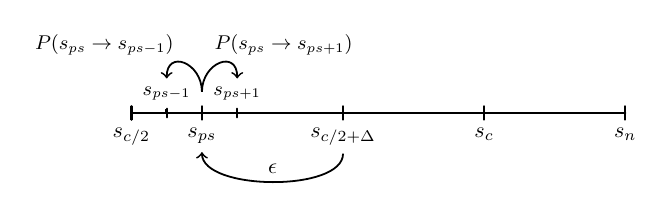
\begin{tikzpicture}[x=1.12cm, scale=0.8, every node/.append style={transform shape}]
    \draw[line width=0.2ex, line cap=round] (0,0) -- (7,0); %edit here for the axis
    \foreach \x in {0,1,3,5,7} % edit here for the vertical lines
    \draw[line width=0.2ex, line cap=round, shift={(\x,0)},color=black] (0pt,3pt) -- (0pt,-3pt);
    \foreach \x in {0.5,1.5} % edit here for the vertical lines
    \draw[line width=0.15ex, line cap=round, shift={(\x,0)},color=black] (0pt,2pt) -- (0pt,-2pt);
    \foreach \x/\y/\z in {
        0/$s_{c/2}$/a,
        1/$s_{ps}$/b,
        3/$s_{c/2+\Delta}$/c,
        5/$s_c$/d,
        7/$s_n$/e}
    \draw[line width=0.2ex, shift={(\x,0)},color=black] (0pt,0pt) -- (0pt,-3pt) node[below] (\z) {\y};
    \foreach \x/\y/\z in {
        0.5/\small$s_{ps-1}$/f,
        1//h,
        1.5/\small$s_{ps+1}$/g}
    \draw[line width=0.2ex, shift={(\x,0)},color=black] (0pt,0pt) -- (0pt,2pt) node[above] (\z) {\y};

    \begin{scope}[line width=0.15ex]
        %\path[->] (c) edge[out=-90, in=-85, looseness=0.7] node[above] {} (d);
        \path[->] (c) edge[out=-90, in=-90, looseness=0.7] node[above] {$\epsilon$} (b);
        \path[->] (h) edge[out=90, in=90, looseness=2] node[above,xshift=-0.5in] {\small$P(s_{ps} \to s_{ps-1})$} (f);
        \path[->] (h) edge[out=90, in=90, looseness=2] node[above,xshift=+0.4in] {\small$P(s_{ps} \to s_{ps+1})$} (g);
    \end{scope}
    %\draw [thick,decoration={brace,raise=1ex, amplitude=2ex},decorate] (5, 0) -- (7, 0) node[midway,above,yshift=3.5ex] {$b$};
\end{tikzpicture}

